\begin{figure}[H]
    \centering
    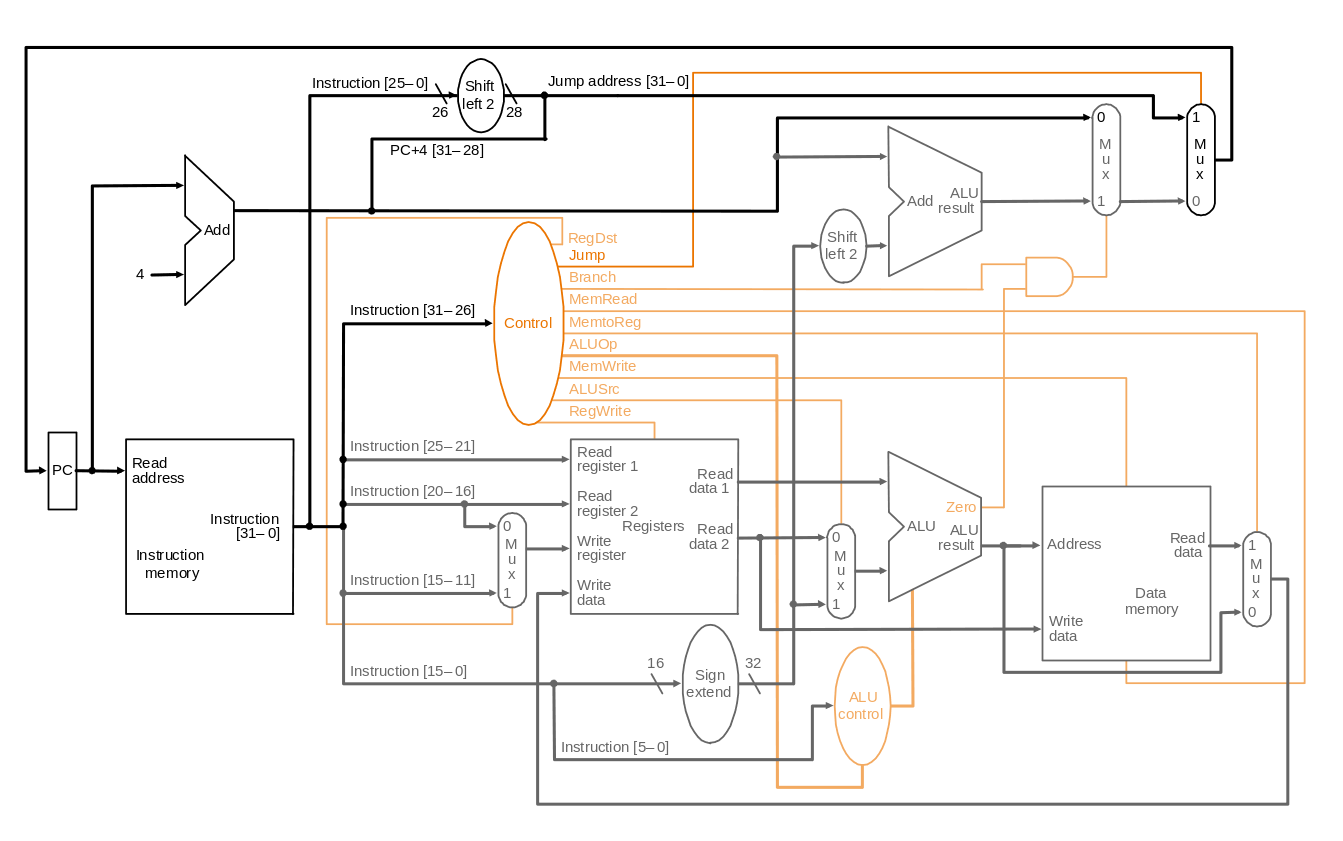
\includegraphics[scale=0.3]{img/single-cycle-cpu.png}
    \caption{Single-cycle CPU with jump and branch.}
    \label{img:single-cycle-cpu}
\end{figure}

\begin{figure}[H]
    \centering
    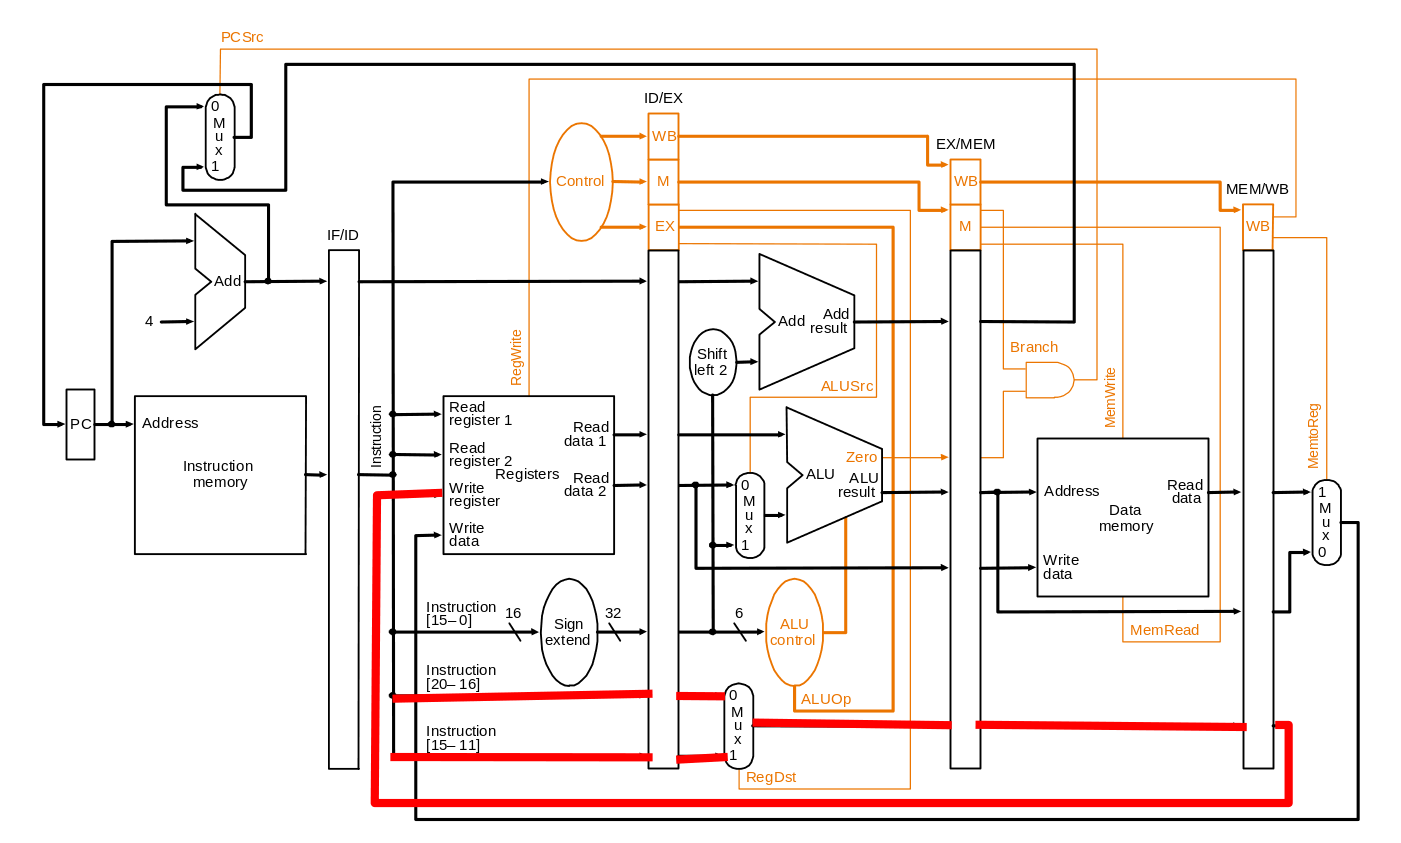
\includegraphics[scale=0.3]{img/pipeline-org.png}
    \caption{Original pipeline.}
    \label{img:pipeline-org}
\end{figure}

\begin{figure}[H]
    \centering
    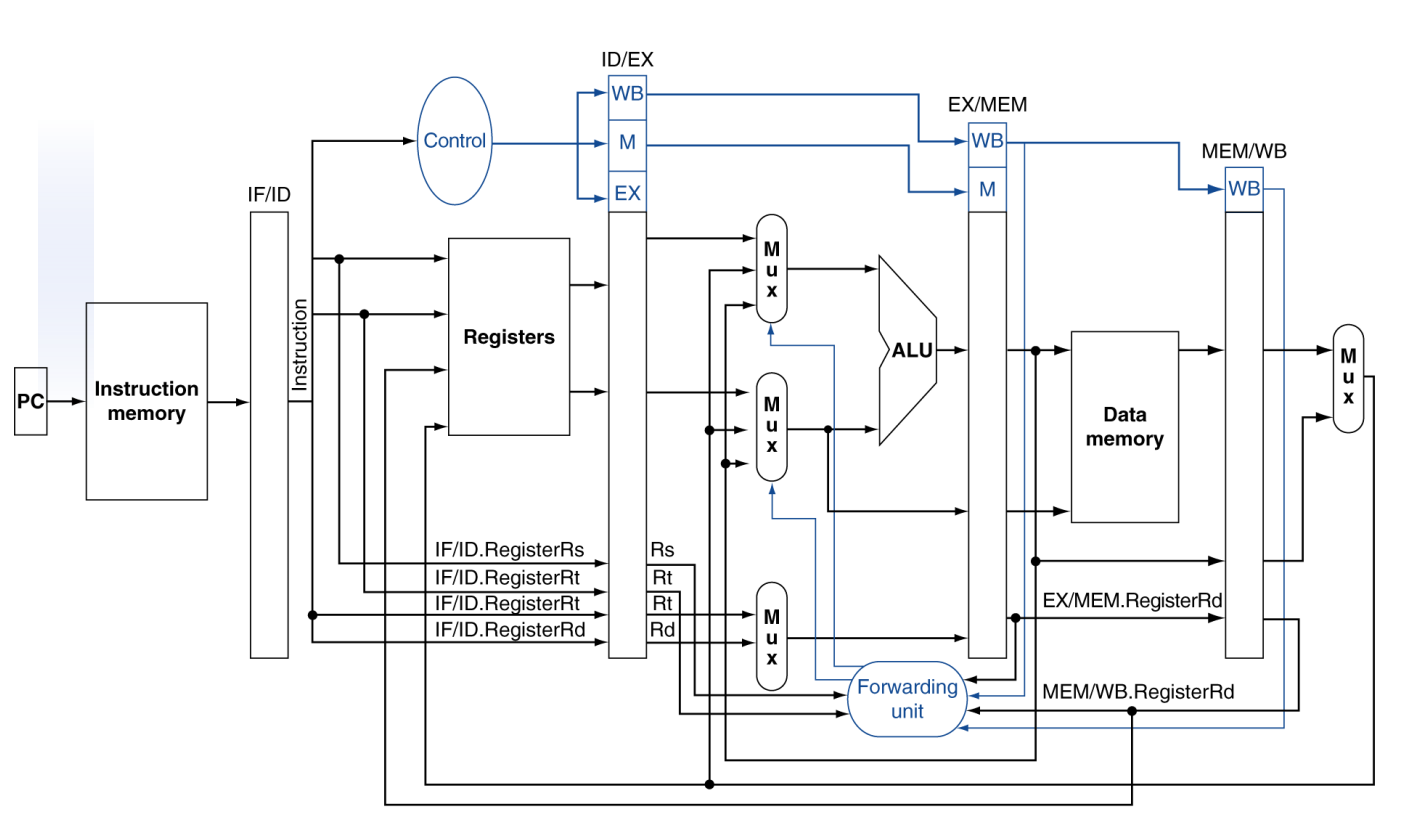
\includegraphics[scale=0.3]{img/pipeline-forward.png}
    \caption{Pipeline with forwarding.}
    \label{img:pipeline-forward}
\end{figure}

\begin{figure}[H]
    \centering
    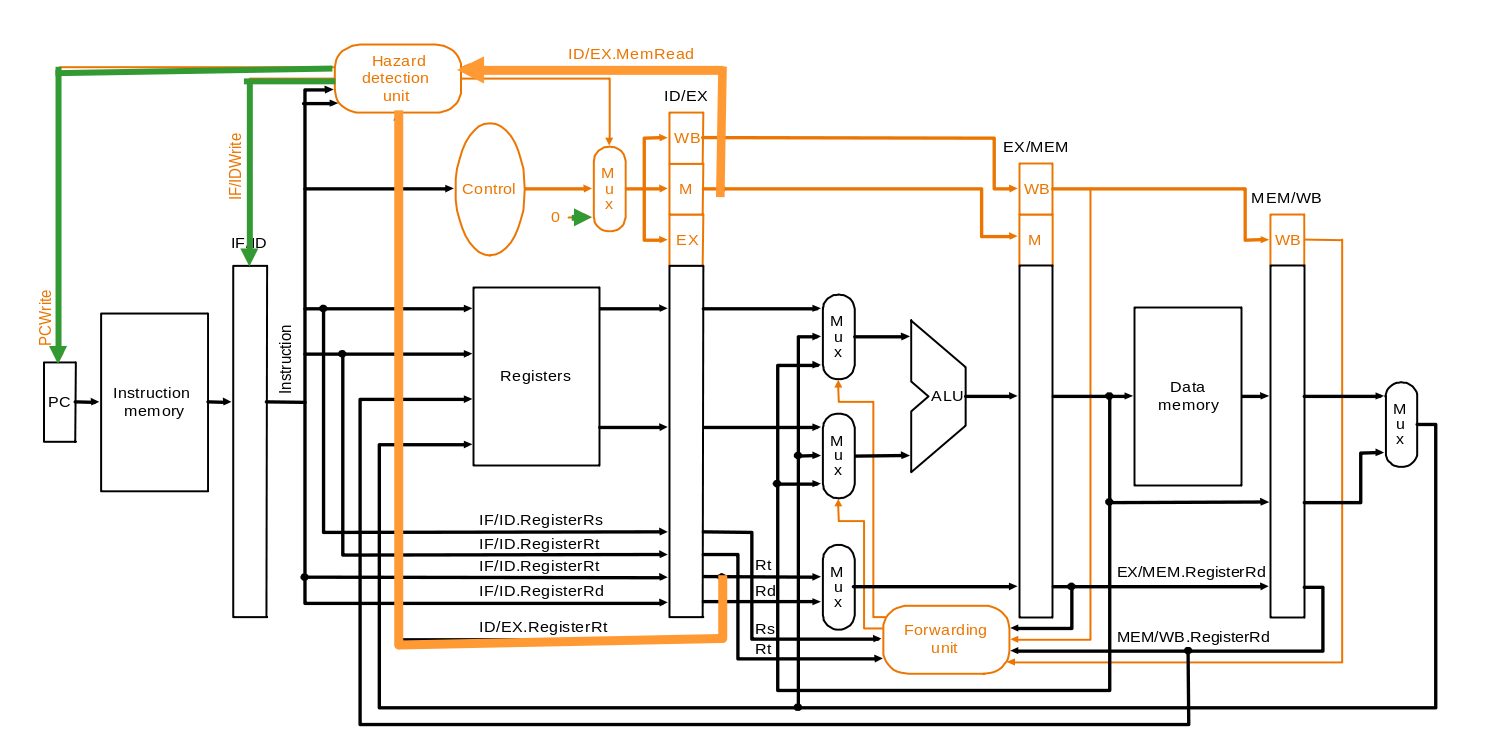
\includegraphics[scale=0.3]{img/pipeline-hazard.png}
    \caption{Pipeline with hazard detection and forwarding units.}
    \label{img:pipeline-hazard}
\end{figure}

\begin{figure}[H]
    \centering
    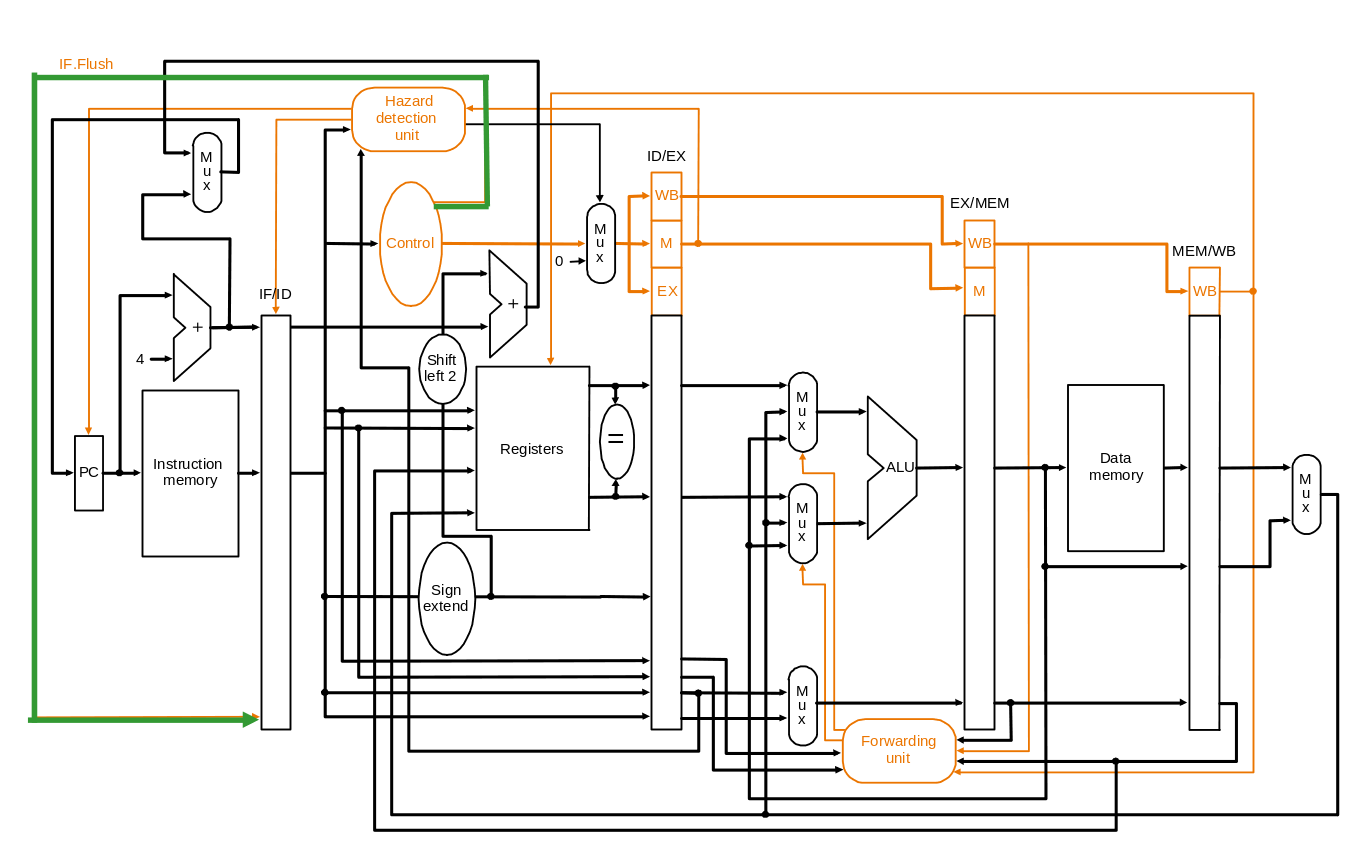
\includegraphics[scale=0.3]{img/pipeline-flush.png}
    \caption{Pipeline with hazard detection, forwarding units and flush.}
    \label{img:pipeline-flush}
\end{figure}

\begin{itemize}
    \item Endianness:\begin{itemize}
        \item Big Endian:最左邊或MSB放在最低address,e.g. MIPS。
        \item Little Endian:最右邊或LSB放在最低address,e.g. x86。
    \end{itemize}
    \item \quad\quad \begin{itemize}
        \item \code{srl/sll rd, rt, shamt # rs = 5'0 }
        \item \code{lw/sw rt, imm(rs)}
        \item \code{beq/bne rs, rt, addr}
        \item \code{addi rt, rs, imm}
        \item \code{lb}: Load最高address(LSB)到最高address(LSB),\code{sb}: Store最高address(LSB)到最低address(MSB)。
        \item \code{jr rs # rt = rd = shamt = 5'0}:R-type
    \end{itemize}
    \item \quad\quad \begin{lstlisting}[language={C}]
        int fact (int n) {
            if (n < 1)
                return 1;
            else
                return (n * fact(n - 1));            
        }
    \end{lstlisting}
    \begin{lstlisting}[language={[x86masm]Assembler}]
        fact:
            addi $sp, $sp, -8
            sw $ra, 4($sp)
            sw $a0, 0($sp)
            slti $t0, $a0, 1
            beq $t0, $zero, L1
            addi $v0, $zero, 1
            addi $sp, $sp, 8
            jr $ra
        L1:
            addi $a0, $a0, -1
            jal fact
            lw $a0, 0($sp)
            lw $ra, 4($sp)
            addi $sp, $sp, 8
            mul $v0, $a0, $v0
            jr $ra
    \end{lstlisting}
    \item 浮點數:
    \begin{table}[H]
        \centering
        \begin{tabular}{|c|c|c|c|c|}
            \hline
            \multicolumn{2}{|c|}{Single precision} & \multicolumn{2}{c|}{Double precision} & Representation \\
            \Xhline{2\arrayrulewidth}
            Exponent & Fraction & Exponent & Fraction & \\
            \hline
            $0$ & $0$ & $0$ & $0$ & $\pm 0$ \\
            \hline
            $0$ & $\neq 0$ & $0$ & $\neq 0$ & $\pm$ denormalized number \\
            \hline
            $1 \sim 254$ & $\texttimes$ & $1 \sim 2046$ & $\texttimes$ & $\pm$ floating-point number \\
            \hline
            $255$ & $0$ & $2047$ & $0$ & $\pm \infty$ \\
            \hline
            $255$ & $\neq 0$ & $2047$ & $\neq 0$ & NaN \\
            \hline
        \end{tabular}
    \end{table}
    \item Overflow detection: \begin{itemize}
        \item 有號數:\begin{lstlisting}[language={[x86masm]Assembler}]
            addu $t0, $t1, $t2
            xor $t3, $t1, $t2 
            slt $t3, $t3, $zero # $t3 = 1 if sign differs
            bne $t3, $zero, NO_OVERFLOW
            xor $t3, $t0, $t1 # Check if the sum sign differs
            slt $t3, $t3, $zero
            bne $t3, $zero, OVERFLOW
        \end{lstlisting}
        \item 無號數:\begin{lstlisting}[language={[x86masm]Assembler}, mathescape=true]
            addu $\text{\$}$t0, $\text{\$}$t1, $\text{\$}$t2
            nor $\text{\$}$t3, $\text{\$}$t1, $\text{\$}$zero # $2^{32} - \$t1 - 1$
            sltu $\text{\$}$t3, $\text{\$}$t3, $\text{\$}$t2 # $2^{32} - \$t1 - 1 < \$t2 \rightarrow 2^{32} - 1 < \$t1 + \$t2$
            bne $\text{\$}$t3, $\text{\$}$zero, OVERFLOW
        \end{lstlisting}
    \end{itemize}
    \item \begin{table}[H]
        \centering
        \begin{tabular}{|c|c|c|}
            \hline
            Instruction & ALUOp1 & ALUOp2 \\
            \Xhline{2\arrayrulewidth}
            \code{lw/sw} & $0$ & $0$ \\
            \hline
            \code{beq} & $\texttimes$ & $1$ \\
            \hline
            R-type & $1$ & $\texttimes$\\
            \hline
        \end{tabular}
    \end{table}
    \item Data hazards:\begin{itemize}
        \item Forwarding:Combinational units,放在$EX$因為ALU。
        \begin{lstlisting}[caption={EX hazard.}, captionpos=b, mathescape=true, language={[x86masm]Assembler}, autogobble=true]
            if (EX/MEM.RegWrite $\land$ (EX/MEM.Rd $\neq 0$) $\land$ 
                (EX/MEM.Rd $=$ ID/EX.Rs/Rt))
                ForwardA/B = $10$
        \end{lstlisting}
        \begin{lstlisting}[caption={MEM hazard.}, captionpos=b, mathescape=true, language={[x86masm]Assembler}, autogobble=true]
            if (MEM/WB.RegWrite $\land$ (MEM/WB.Rd $\neq 0$) $\land$ 
                ($\lnot$ EX_hazard) $\land$ (MEM/WB.Rd $=$ ID/EX.Rs/Rt))
                ForwardA/B = $01$
        \end{lstlisting}
        \item Stall:\code{}
        \begin{lstlisting}[caption={Stall.}, captionpos=b, mathescape=true, language={[x86masm]Assembler}, autogobble=true]
            if (ID/EX.MemRead $\land$ (ID/EX.Rt $=$ IF/ID.Rs/Rt))
                IF/ID.Write := $0$
                PC.Write := $0$
        \end{lstlisting}
    \end{itemize}
    \item Control hazards:\begin{itemize}
        \item 若分支指令與\textbf{前一個ALU指令}或\textbf{前面第二個}\code{lw}有data dependency,必須stall $1$ CC。
        \item 分支指令通過\code{xor}再\code{nor}比較是否相同。
        \item Delayed branch:\begin{itemize}
            \item NOT suitable for deep pipeline.
            \item From before:最佳方法,不管跳或不跳皆提升。
            \item From target:用於branch發生機率高,有跳才提升。
            \item From fall through:用於branch發生機率低,不跳才提升。
            \begin{figure}[H]
                \centering
                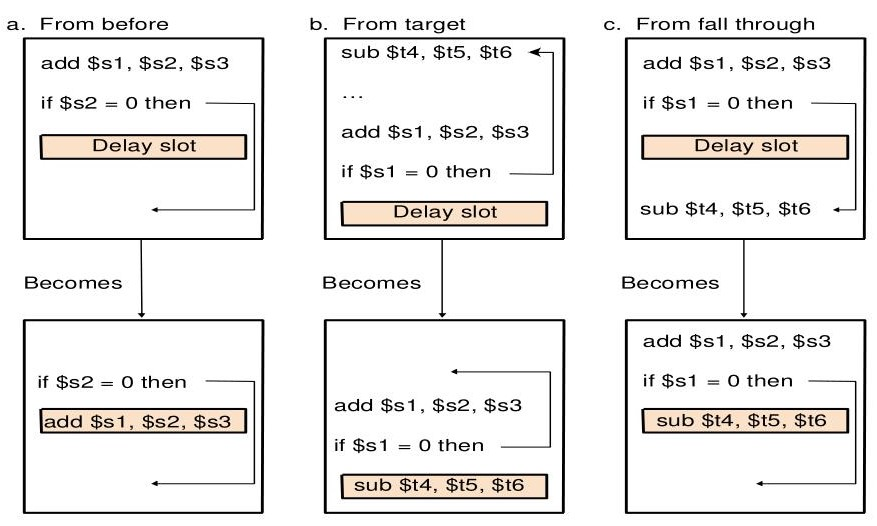
\includegraphics[scale=0.6]{img/delayed-branch.jpg}
                \caption{Example of delayed branch.}
                \label{img:delayed-branch}
            \end{figure}
        \end{itemize}
    \end{itemize}
    \item \quad\quad \begin{itemize}
        \item Intel IA-64 (EPIC):\begin{itemize}
            \item 支援利用compiler開發的平行度。
            \item 可以猜測,並利用if-else取代branch。
            \item Registers比MIPS多很多。
            \item Instruction group is a sequence of instructions which does \textbf{NOT} have data dependency and can be executed parallelly.
        \end{itemize}
        \item Speculation錯誤復原:\begin{itemize}
            \item 軟體提供修補程式。
            \item 硬體CPU將猜測結果暫時儲存,若正確,則將猜測結果寫回register或memory,否則flush buffer。
        \end{itemize}
        \begin{table}[H]
            \centering
            \begin{tabular}{|c|c|c|}
                \hline
                \multicolumn{3}{|c|}{Advanced pipeline} \\
                \Xhline{3\arrayrulewidth}
                Technique & Hardware & Software \\
                \Xhline{2\arrayrulewidth}
                Branch prediction & $\surd$ & $\surd$ \\
                \hline
                Speculation & $\surd$ & $\surd$ \\
                \hline
                Intel IA-64 (EPIC) & $\surd$ & $\surd$ \\
                \hline
                Register renaming & $\surd$ & $\surd$ \\
                \hline
                Prediction & & $\surd$ \\
                \hline
            \end{tabular}
        \end{table}
    \end{itemize}
    \item MIPS exception handling: \begin{itemize}
        \item Flush the instruction and let all preceding instructions complete if they can.
        \item 利用cause register儲存exception原因。
        \item 將造成exception的instruction memory address存在EPC ($PC + 4$)。
        \item 使用entry point switch to kernel。
        \item Exception handling routine須將$PC - 4$。
    \end{itemize}
    \item Non-blocking cache: \begin{itemize}
        \item Does \textbf{NOT} allow \textbf{miss under hit} to hide miss latency. 
        \item \textbf{Miss under miss} allows multiple outstanding cache misses.
        \item Allow a \textbf{load} instruction to access the cache if the previous \textbf{load} is a cache miss.
    \end{itemize}
    \item RAID:\begin{itemize}
        \item RAID 2:Hamming code,Write需要讀取所有disks,從新計算Hamming code並寫入ECC disks,效率差,$2n - 1$ disks。
        \item RAID 3:\begin{itemize}
            \item Reliability和RAID 2相同。
            \item 不做備份,花費較多時間恢復data,$n + 1$ disks。
            \item 當$1$個disk出錯可救回來,多個則否。
            \item Availability cost為$\frac{1}{N}$,其中$N$為protection group disks數量。
            \item Parity集中存放一個disk。
        \end{itemize}
        \item RAID 4:\begin{itemize}
            \item 只對protection group其中一disk做small reads。
            \item $n + 1$ disks,parity集中存放一個disk。
            \item 當$1$個disk出錯可救回來,多個則否。
        \end{itemize}
        \item RAID 5:\begin{itemize}
            \item Write就不會有單一disk瓶頸。
            \item $n + 1$ disks,parity被分散到所有disks。
            \item 可允許$1$個disk故障。
        \end{itemize}
        \item RAID 6:\begin{itemize}
            \item 與RAID 5相比,增加第二個獨立的parity block。
            \item 通常通過硬體實現。
            \item $n + 2$ disks。
            \item 可允許$2$個disk故障。
        \end{itemize}
        \item RAID 3 has \textbf{worst} throughput for \textbf{small writes}.
        \item RAID 3 has \textbf{best small writes latency}.
        \item RAID 3, 4, 5 have same throughput for \textbf{large writes}.
        \item RAID 1 can \textbf{NOT} have \textbf{small writes} in parallel.
        \item RAID 3 can \textbf{NOT} have \textbf{small writes or reads} in parallel. 
        \item RAID 4, 5 perform same for parallel \textbf{small reads and writes}. 
        \item RAID 4 does \textbf{NOT} have better \textbf{big reads} performance than RAID 3.
        \item RAID 1+0 has better \textbf{write throughput} than RAID 0+1.
    \end{itemize}
    \item \quad\quad \begin{figure}[H]
        \centering
        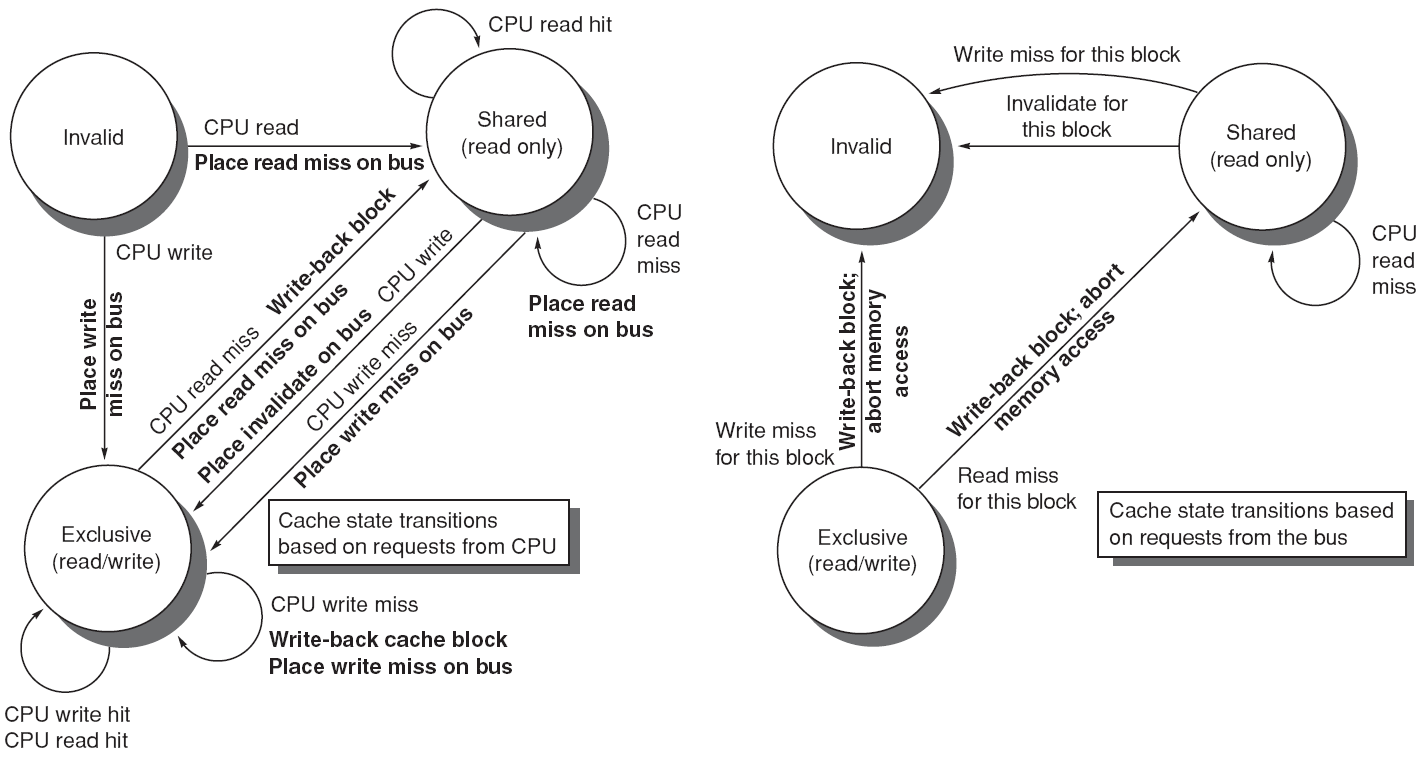
\includegraphics[scale=0.5]{img/snooping.png}
        \caption{Snooping states.}
        \label{img:snooping}
    \end{figure}
    \item Multithreading: \begin{itemize}
        \item Coarse-grained multithreading: Switch threads only on costly stalls, such as L2 cache misses. Pipeline \textbf{start-up} costs.
        \item Fine-grained multithreading: Switch between threads on each instruction packs. It can hide the throughput losses.
        \item SMT: \textbf{ILP} and \textbf{TLP}; coarse-grained and fine-grained: \textbf{TLP only}.
    \end{itemize}
    \item Network topology: \begin{itemize}
        \item Performance measure:\begin{itemize}
            \item Network bandwidth.
            \item Bisection bandwidth:平均切為二所減少的bandwidth,越高容錯力越高。
            \item Diameter:任兩點最短路的最大值,越低越好。
            \item Nodal degree:CPU degree,越高容錯力越高。
        \end{itemize}
        \item Omega network hardware: $2n\log_2 n$.
        \item Crossbar network hardware: $n^2$.
    \end{itemize}
    \item \quad\quad \begin{itemize}
        \item Time-sharing (Multitasking):使用virtual memory以及spooling,且對所有users公平對待。
        \item Real-time:\begin{itemize}
            \item \textbf{Hard} real-time disk少用,\textbf{不}使用virtual memory;但\textbf{soft} real-time可,但real-time processes的pages在完成前不能被swapped out。
            \item \textbf{Hard} real-time\textbf{不}與time-sharing並存;但\textbf{soft} real-time可。
            \item 減少kernel干預時間,因為Linux kernel在執行某些system process時,\textbf{不}允許user process preempts kernel,防止race condition。
        \end{itemize}
    \end{itemize}
    \item \quad\quad \begin{itemize}
        \item Interrupt:Hardward-generated, e.g. I/O-complete, Time-out.
        \item Trap:Software-generated。Catch arithmetic error或重大error,例如Divide-by-zero,以及process需要OS提供服務,會先發trap通知OS。
    \end{itemize}
    \item Scheduler:\begin{itemize}
        \item Long-term (Job) scheduler:通常僅\textbf{batch system採用},從job queue中選jobs載入memory。執行頻率最低,可以調控multiprogramming degree與CPU-bound與I/O-bound jobs的比例。
        \item Short-term (CPU, process) scheduler:從ready queue選擇一個process分派給CPU執行。\textbf{所有系統都需要},執行頻率最高,\textbf{無法}調控multiprogramming degree與CPU-bound與I/O-bound jobs的比例。
        \item Medium-term scheduler:Memory space不足且有其他processes需要更多memory時執行,選擇Blocked或lower priority process swap out to disk。僅\textbf{Time-sharing system採用},batch和real-time systems不採用,可以調控multiprogramming degree與CPU-bound與I/O-bound jobs的比例。
    \end{itemize}
    \item Dispatcher: \begin{itemize}
        \item 將CPU真正分配給CPU scheduler選擇的process。
        \item Context switching.
        \item Switch mode to user mode.
        \item Jump to execution entry of user process.
    \end{itemize}
    \item CPU scheduling: \begin{itemize}
        \item Non-preemptive SJF\textbf{不}適合用在\textbf{short-term} scheduler,因為很難在短時間算出next CPU burst;long-term scheduler較合適。
        \item MFQ雖然不公平,但\textbf{NO} starvation。
        \item Linux指定processes\textbf{不要}移轉到某些processors。
        \item Worst-case CPU utilization for scheduling $n$ processes using Rate-monotonic: \begin{equation}
            \begin{aligned}
                & 2 \times (2^{\frac{1}{n}} - 1) \\
                \Rightarrow & \ (n \rightarrow \infty) = 69\%
            \end{aligned}
        \end{equation}
        \item Dispatch latency:\begin{itemize}
            \item Conflict phase:preempts kernel,並且low-priority process releases needed resources for high-priority process。
            \item Dispatch phase:Context switching, change mode to user mode, and jump to the user process.
        \end{itemize}
    \end{itemize}
    \item Deadlock avoidance:\begin{itemize}
        \item 若$n$ processes,$m$ resources(單一種類),若滿足\begin{equation} \label{eq:deadlock}
            \begin{aligned}
                1 \le \ & Max_i \le m \\
                & \sum_{i = 1}^{n} Max_i < n + m
            \end{aligned}
        \end{equation} 則NO deadlock。\\ \begin{proof}
            若所有資源都分配給processes,即\begin{equation}
                \sum_{i = 1}^{n} Allocation_i = m
            \end{equation} 又\begin{equation}
                \begin{aligned}
                    & \sum_{i = 1}^{n} Need_i = \sum_{i = 1}^{n} Max_i - \sum_{i = 1}^{n} Allocation_i \\
                    \rightarrow & \sum_{i = 1}^{n} Max_i = \sum_{i = 1}^{n} Need_i + m
                \end{aligned}
            \end{equation}
            根據第二條件,有\begin{equation}
                \begin{aligned}
                    & \sum_{i = 1}^{n} Max_i < n + m \\
                    \rightarrow & \sum_{i = 1}^{n} Need_i < n
                \end{aligned}
            \end{equation}$\exists$ process $P_i$,$Need_i = 0$,又\begin{equation}
                \begin{aligned}
                    & Max_i \ge 1 \land Need_i = 0 \\
                    \rightarrow & Allocation_i \ge 1
                \end{aligned}
            \end{equation}在$P_i$完工後,會產生$\ge 1$ resources給其他processes使用,又可以使$\ge 1$ processes $P_j$有$Need_j = 0$,依此類推,所有processes皆可完工。
        \end{proof}
    \end{itemize}
    \item Critical section: \begin{itemize}
        \item 在critical section,CPU也可能被preempted。
        \item 滿足:\begin{itemize}
            \item Mutual exclusion:同一時間點,最多$1$ process在他的critical section,不允許多個processes同時在\textbf{各自}的critical section。
            \item Progress:不想進入critical section時,不能阻礙其他想進入critcal section的process進入,即不能參與進入critical section的decision,且必須在有限時間內決定進入critical section的process。
            \item Bounded waiting:Process提出申請進入critical section後,必須在有限時間內進入,即公平,NO starvation。
        \end{itemize}
    \end{itemize}
    \item Two processes solution (Peterson's solution):\begin{itemize}
        \item 共享變數:\begin{lstlisting}[caption={Shared variables of Peterson's solution (two processes solution).}, captionpos=b, mathescape=true]
            int turn = $i \lor j$;
            bool flag = $False$;
        \end{lstlisting}
        \item $flag$或$turn$或兩者值皆互換依然正確,但若將前兩行賦值順序對調,則因為\textbf{mutual exclusion不成立},而不正確。
        \item Peterson's solution is NOT guaranteed to work on modern PC, since processors and compilers may reorder read and write operations that have NO dependencies.
        \begin{algorithm}[H]
            \caption{$P_i$ of Peterson's solution (two processes solution).}
            \begin{algorithmic}[1]
                \Function{$P_i$}{}
                    \Repeat 
                        \State $flag[i]$ := $True$
                        \State $turn$ := $j$
                        \While {$flag[j] \land turn = j$}
                        \EndWhile
                        \State Critacal section.
                        \State $flag[i]$ := $False$
                        \State Remainder section.
                    \Until {$False$}
                \EndFunction
            \end{algorithmic}
        \end{algorithm}
    \end{itemize}
    \item Test-and-Set:\begin{itemize}
        \item 共享變數:\begin{lstlisting}[caption={Shared variables of \textsc{Test-and-Set} solution.}, captionpos=b, mathescape=true]
            bool lock = $False$;
            /*
            True,表示想進但在等;
            False,表示已在critical section或是初值。
            */
            bool waiting[$0 \ \cdots \ (n - 1)$] = $False$;
        \end{lstlisting}
        \item 若移除第八行\code{waiting[i] := False},則\textbf{progress不成立},若僅$P_i$和$P_j$想進入critical section,此時\code{waiting[i], waiting[j] = True},且$P_i$先進入critical section,有\code{lock, waiting[i] = True};
        當$P_i$離開critical section後,將\code{waiting[j] := False},$P_j$進入critical section;當$P_j$離開critical section後,因為\code{waiting[i] = True},$P_j$將\code{waiting[i] := False},但\code{lock = True},未來沒有process可以再進入critical section,\textbf{deadlock}。
        \begin{algorithm}[H]
            \caption{$P_i$ (Test-and-Set).}
            \label{algo:test-and-set-algo-2}
            \begin{algorithmic}[1]
                \Function{$P_i$}{}
                    \Repeat
                        \State $waiting[i]$ := $True$
                        \State $key$ := $True$ \Comment{Local variable.}
                        \While {$waiting[i] \land key$}
                            \State $key$ := \Call{Test-and-Set}{$\& lock$}
                        \EndWhile
                        \State $waiting[i]$ := $False$
                        \State Critical section.
                        \State $j$ := $i + 1 \Mod{n}$
                        \While {$j \neq i \land \lnot waiting[j]$} \Comment{找下一個想進入的$P_j$。}
                            \State $j$ := $j + 1 \Mod{n}$
                        \EndWhile
                        \If {$j = i$} \Comment{沒有$P_j$想進入critical section。}
                            \State $lock$ := $False$
                        \Else 
                            \State $waiting[j]$ := $False$
                        \EndIf
                        \State Remainder section.
                    \Until {$False$}
                \EndFunction
            \end{algorithmic}
        \end{algorithm}
    \end{itemize}
    \item Producer-consumer problem:\begin{itemize}
        \item 共享變數:\begin{lstlisting}[caption={Shared variables of Producer-consumer problem.}, captionpos=b, mathescape=true]
            semaphore mutex = $1$;
            semaphore empty = $n$; // buffer空格數。
            semaphore full = $0$; // buffer中item數。
        \end{lstlisting}
        \item 若將其中一個或兩個程式的兩行\code{wait}對調,可能會\textbf{deadlock}。
        \begin{algorithm}[H]
            \caption{Producer.}
            \begin{algorithmic}[1]
                \Function{Producer}{}
                    \Repeat
                        \State Produce an item.
                        \State \Call{wait}{$empty$}
                        \State \Call{wait}{$mutex$}
                        \State Add the item to buffer.
                        \State \Call{signal}{$mutex$}
                        \State \Call{signal}{$full$}
                    \Until {$False$}
                \EndFunction
            \end{algorithmic}
        \end{algorithm}
        \begin{algorithm}[H]
            \caption{Consumer.}
            \begin{algorithmic}[1]
                \Function{Consumer}{}
                    \Repeat
                        \State \Call{wait}{$full$}
                        \State \Call{wait}{$mutex$}
                        \State Retrieve an item from buffer.
                        \State \Call{signal}{$mutex$}
                        \State \Call{signal}{$empty$}
                        \State Consume the item.
                    \Until {$False$}
                \EndFunction
            \end{algorithmic}
        \end{algorithm}
    \end{itemize}
    \item Reader/Writer problem:\begin{itemize}
        \item R/W和W/W皆要互斥。
        \item First readers/writers problem:\begin{itemize}
            \item 共享變數:\begin{lstlisting}[caption={Shared variables of First Reader/Writer problem.}, captionpos=b, mathescape=true]
                // R/W和W/W互斥控制,同時對writer不利之阻擋。
                semaphore wrt = $1$ ;
                int readcnt = $0$;
                semaphore mutex = $1$; // readcnt互斥控制。
            \end{lstlisting}
        \end{itemize}
        \begin{algorithm}[H]
            \caption{Writer (First Reader/Writer problem).}
            \begin{algorithmic}[1]
                \Function{Writer}{}
                    \Repeat
                        \State \Call{wait}{$wrt$}
                        \State Writing.
                        \State \Call{signal}{$wrt$}
                    \Until {$False$}
                \EndFunction
            \end{algorithmic}
        \end{algorithm}
        \begin{algorithm}[H]
            \caption{Reader (First Reader/Writer problem).}
            \begin{algorithmic}[1]
                \Function{Reader}{}
                    \Repeat
                        \State \Call{wait}{$mutex$}
                        \State $readcnt$ := $readcnt + 1$
                        \If {$readcnt = 1$} \Comment{表示第一個reader需偵測有無writer在。}
                            \State \Call{wait}{$wrt$} 
                        \EndIf
                        \State \Call{signal}{$mutex$} 
                        \State Reading.
                        \State \Call{wait}{$mutex$}
                        \State $readcnt$ := $readcnt - 1$
                        \If {$readcnt = 0$} \Comment{No reader.}
                            \State \Call{signal}{$wrt$} 
                        \EndIf
                        \State \Call{signal}{$mutex$}
                    \Until {$False$}
                \EndFunction
            \end{algorithmic}
        \end{algorithm}
        \item Second Reader/Writer problem:\begin{itemize}
            \item 共享變數:\begin{lstlisting}[caption={Shared variables of Second Reader/Writer problem.}, captionpos=b, mathescape=true]
                int readcnt = $0$;
                semaphore mutex = $1$; // readcnt互斥控制。
                semaphore wrt = $1$; // R/W和W/W互斥控制。
                int wrtcnt = $0$;
                semaphore y = $1$; // wrtcnt互斥控制。
                semaphore rsem = $1$; // 對reader不利之阻擋。
                semaphore z = $1$; // reader的入口控制,可有可無。
            \end{lstlisting}
        \end{itemize}
        \begin{algorithm}[H]
            \caption{Writer (Second Reader/Writer problem).}
            \begin{algorithmic}[1]
                \Function{Writer}{}
                    \Repeat
                        \State \Call{wait}{$y$} 
                        \State $wrtcnt$ := $wrtcnt + 1$
                        \If {$wrtcnt = 1$} \Comment{表示第一個writer需阻擋readers。}
                            \State \Call{wait}{rsem}
                        \EndIf
                        \State \Call{signal}{$y$}
                        \State \Call{wait}{$wrt$}
                        \State Writing.
                        \State \Call{wait}{$y$}
                        \State $wrtcnt$ := $wrtcnt - 1$
                        \If {$wrtcnt = 0$}
                            \State \Call{signal}{rsem} \Comment{No writer.}
                        \EndIf
                        \State \Call{signal}{$wrt$}
                        \State \Call{signal}{$y$}
                    \Until {$False$}
                \EndFunction
            \end{algorithmic}
        \end{algorithm}
        \begin{algorithm}[H]
            \caption{Reader (Second Reader/Writer problem).}
            \begin{algorithmic}[1]
                \Function{Reader}{}
                    \Repeat
                        \State \Call{wait}{$z$} 
                        \State \Call{wait}{$rsem$} 
                        \State \Call{wait}{$mutex$}
                        \State $readcnt$ := $readcnt + 1$
                        \If {$readcnt = 1$}
                            \State \Call{wait}{$wrt$}
                        \EndIf
                        \State \Call{signal}{$mutex$}
                        \State \Call{signal}{$rsem$} 
                        \State \Call{signal}{$z$} 
                        \State Reading.
                        \State \Call{wait}{$mutex$}
                        \State $readcnt$ := $readcnt - 1$
                        \If {$readcnt = 0$}
                            \State \Call{signal}{$wrt$}
                        \EndIf
                        \State \Call{signal}{$mutex$}
                    \Until {$False$}
                \EndFunction
            \end{algorithmic}
        \end{algorithm}
    \end{itemize}
    \item The sleeping barber problem:\begin{itemize}
        \item 共享變數:\begin{lstlisting}[caption={Shared variables of The sleeping barber problem.}, captionpos=b, mathescape=true]
            semaphore customer = $0$; // 強迫barber sleep。
            // 強迫customer sleep if barber is busy。
            semaphore barber = $0$; 
            int waiting = $0$; // 正在等待的customers個數。
            semaphore mutex = $1$; // waiting互斥控制。
        \end{lstlisting}
        \item 若將\textsc{Barber}將兩行\code{wait}對調,可能會\textbf{deadlock}。
        \begin{algorithm}[H]
            \caption{Barber.}
            \begin{algorithmic}[1]
                \Function{Barber}{}
                    \Repeat
                        \State \Call{wait}{$customer$} \Comment{Barber go to sleep if no customer.}
                        \State \Call{wait}{$mutex$}
                        \State $waiting$ := $waiting - 1$
                        \State \Call{signal}{$barber$} \Comment{Wake up customer.}
                        \State \Call{signal}{$mutex$}
                        \State Cutting hair.
                    \Until {$False$}
                \EndFunction
            \end{algorithmic}
        \end{algorithm}
        \begin{algorithm}[H]
            \caption{Customer.}
            \begin{algorithmic}[1]
                \Function{Customer}{}
                    \Repeat
                        \State \Call{wait}{$mutex$}
                        \If {$waiting < n$} \Comment{入店。}
                            \State $waiting$ := $waiting + 1$
                            \State \Call{signal}{$customer$} \Comment{Wake up barber.}
                            \State \Call{signal}{$mutex$}
                            \State \Call{wait}{$barber$} \Comment{Customer go to sleep if barber is busy.}
                            \State Getting cut.
                        \Else
                            \State \Call{signal}{$mutex$}
                        \EndIf
                    \Until {$False$}
                \EndFunction
            \end{algorithmic}
        \end{algorithm}
    \end{itemize}
    \item The dining-philosophers problem:\begin{itemize}
        \item 五位哲學家兩兩間放一根筷子吃中餐(筷子),哲學家需取得左右兩根筷子才能吃飯。若吃西餐(刀叉),必須\textbf{偶數}個哲學家,
        \item Algorithm 1:\begin{itemize}
            \item 根據公式 (\ref{eq:deadlock}),人數必須$< 5$才不會deadlock。
            \item 共享變數:\begin{lstlisting}[caption={Shared variables of The dining-philosophers problem.}, captionpos=b, mathescape=true]
                semaphore chopstick[$0 \ \cdots \ 4$] = $1$;
                // 可拿筷子的哲學家數量互斥控制。
                semaphore no = $4$; 
            \end{lstlisting}
            \begin{algorithm}[H]
                \caption{$P_i$ of Algorithm 1 (The dining-philosophers problem).}
                \begin{algorithmic}[1]
                    \Function{$P_i$}{}
                        \Repeat
                            \State \Call{wait}{$no$}
                            \State Hungry.
                            \State \Call{wait}{$chopstick[i]$}
                            \State \Call{wait}{$chopstick[(i + 1 \Mod{5})]$}
                            \State Eating.
                            \State \Call{signal}{$chopstick[i]$}
                            \State \Call{signal}{$chopstick[(i + 1 \Mod{5})]$}
                            \State Thinking.
                            \State \Call{signal}{$no$}
                        \Until {$False$}
                    \EndFunction
                \end{algorithmic}`'
            \end{algorithm}
        \end{itemize}
        \item Algorithm 2:只有能夠同時拿左右兩根筷子才允許持有筷子,否則不可持有任何筷子,\textbf{破除hold and wait},不會deadlock。
        \item Algorithm 3:當有\textbf{偶數}個哲學家時,偶數號的哲學家先取左邊,再取右邊,奇數號的則反之,\textbf{破除circular wait},不會deadlock。與吃西餐先拿刀再拿叉相似。
    \end{itemize}
    \item Binary semaphore製作counting semaphore(若為$-n$表示$n$個process卡在\code{wait}):\begin{itemize}
        \item 共享變數:\begin{lstlisting}[caption={Shared variables of The dining-philosophers problem.}, captionpos=b, mathescape=true]
            int c = $n$; // Counting semaphore號誌值。
            semaphore $s_1$ = $1$; // $c$互斥控制。
            binary_semaphore $s_2$ = $0$; // $c < 0$時卡住process
        \end{lstlisting}
        \begin{algorithm}[H]
            \caption{$wait(c)$ (counting semaphore).}
            \begin{algorithmic}[1]
                \Function{wait}{$c$}
                    \State \Call{wait}{$s_1$}
                    \State $c$ := $c - 1$
                    \If {$c < 0$}
                        \State \Call{signal}{$s_1$}
                        \State \Call{wait}{$s_2$} \Comment{Process卡住。}
                    \Else
                        \State \Call{signal}{$s_1$}
                    \EndIf
                \EndFunction
            \end{algorithmic}
        \end{algorithm}
        \begin{algorithm}[H]
            \caption{$signal(c)$ (counting semaphore).}
            \begin{algorithmic}[1]
                \Function{signal}{$c$}
                    \State \Call{wait}{$s_1$}
                    \State $c$ := $c + 1$
                    \If {$c \le 0$} \Comment{先前有process卡住。}
                        \State \Call{signal}{$s_2$}
                    \EndIf
                    \State \Call{signal}{$s_1$}
                \EndFunction
            \end{algorithmic}
        \end{algorithm}
    \end{itemize}
    \item Process is NOT active:\begin{itemize}
        \item Process呼叫的function執行完畢。
        \item Process執行\code{wait()}被blocked。
    \end{itemize}
    \item  Monitor解The dining philosophers problem:
    \begin{lstlisting}[caption={Data structure (The dining philosophers problem (Monitor)).}, captionpos=b, mathescape=true]
        Monitor Dining-ph {
            enum {
                thinking, hungry, eating
            } state[5];
        } 
        Condition self[5];
    \end{lstlisting}
    \begin{algorithm}[H]
        \caption{$pickup(i)$.}
        \begin{algorithmic}[1]
            \Function{pickup}{$i$}
                \State $state[i]$ := $hungry$
                \State \Call{test}{i}
                \If {$state[i] \neq eating$}
                    \State \Call{$self[i]$.wait}{}
                \EndIf
            \EndFunction
        \end{algorithmic}
    \end{algorithm}
    \begin{algorithm}[H]
        \caption{$test(i)$.}
        \begin{algorithmic}[1]
            \Function{test}{$i$}
                \If {$state[(i + 4) \Mod{5}] \neq eating \land state[i] = hungry \land state[(i + 1) \Mod{5}] \neq eating$}
                    \State $state[i]$ := $eating$
                    \State \Call{$self[i]$.signal}{}
                \EndIf
            \EndFunction
        \end{algorithmic}
    \end{algorithm}
    \begin{algorithm}[H]
        \caption{$putdown(i)$.}
        \begin{algorithmic}[1]
            \Function{putdown}{$i$}
                \State $state[i]$ := $thinking$
                \State \Call{test}{$(i + 4) \Mod{5}$}
                \State \Call{test}{$(i + 1) \Mod{5}$}
            \EndFunction
        \end{algorithmic}
    \end{algorithm}
    \begin{algorithm}[H]
        \caption{$initialization\_code()$.}
        \begin{algorithmic}[1]
            \Function{initialization\_code}{} \Comment{For non-Condition type.}
                \For {$i$ := $0$ to $4$}
                    \State $state[i]$ := $thinking$
                \EndFor
            \EndFunction
        \end{algorithmic}
    \end{algorithm}
    \begin{algorithm}[H]
        \caption{$P_i$ (The dining philosophers problem (Monitor)).}
        \begin{algorithmic}[1]
            \Function{$P_i$}{}
                \State \Call{Dining\_ph}{} $dp$ \Comment{Shared variable.}
                \Repeat
                    \State Hungry. \Comment{No active.}
                    \State \Call{$dp$.pickup}{$i$} \Comment{Running: active; Blocked: NOT active.}
                    \State Eating. \Comment{No active.}
                    \State \Call{$dp$.putdown}{$i$} \Comment{Active.}
                    \State Thinking. \Comment{No active.}
                \Until {$False$}
            \EndFunction
        \end{algorithmic}
    \end{algorithm}
    \item 使用semaphore製作monitor:\begin{itemize}
        \item 共享變數:\begin{lstlisting}[caption={Shared variables of making monitor using semaphore.}, captionpos=b, mathescape=true]
            semaphore mutex = $1$;
            // Block process P if P call signal. 
            semaphore next = $0$;
            // 統計process P 那種特殊waiting processes的個數。 
            int next_cnt = $0$;
            // Block process Q if Q call wait.
            semaphore x_sem = $0$;
            // 統計一般waiting processes的個數。
            int x_cnt = $0$; 
        \end{lstlisting}
        \item 在function body前後加入控制碼,類似Entry section和Exit section。
        \begin{algorithm}[H]
            \caption{$f$ (Example for adding control code before and after function body).}
            \begin{algorithmic}[1]
                \Function{f}{}
                    \State \Call{wait}{$mutex$}
                    \State Function body.
                    \If {$next\_cnt > 0$}
                        \State \Call{signal}{$next$}
                    \Else
                        \State \Call{signal}{$mutex$}
                    \EndIf
                \EndFunction
            \end{algorithmic}
        \end{algorithm}
        \begin{algorithm}[H]
            \caption{$x.wait$.}
            \begin{algorithmic}[1]
                \Function{$x$.wait}{}
                    \State $x\_cnt$ := $x\_cnt + 1$
                    \If {$next\_cnt > 0$}
                        \State \Call{signal}{$next$}
                    \Else
                        \State \Call{signal}{$mutex$}
                    \EndIf
                    \State \Call{wait}{$x\_sem$} \Comment{$Q$自己卡住。}
                    \State $x\_cnt$ := $x\_cnt - 1$ \Comment{$Q$被救。}
                \EndFunction
            \end{algorithmic}
        \end{algorithm}
        \begin{algorithm}[H]
            \caption{$x.signal$.}
            \begin{algorithmic}[1]
                \Function{$x$.signal}{}
                    \If {$x\_cnt > 0$}
                        \State $next\_cnt$ := $next\_cnt + 1$
                        \State \Call{signal}{$x\_sem$}
                        \State \Call{wait}{$next$} \Comment{$P$自己卡住。}
                        \State $next\_cnt$ := $next\_cnt - 1$ \Comment{$P$被救。}
                    \EndIf
                \EndFunction
            \end{algorithmic}
        \end{algorithm}
    \item \quad\quad \begin{itemize}
        \item Dynamic binding由MMU負責。
        \item Dynamic loading由programmer負責,OS無負擔。
        \item Dynamic linking需要OS支持。
        \item 必須支援dynamic binding才可以在execution time compaction。
    \end{itemize}
    \item Process可分配frames數量由hardware決定,最多為physical memory size,最少須讓任一machine code完成,即週期中最多可能memory access數量,e.g. $IF$, $MEM$, $WB$共三次。
    \item Dirty bit:\begin{itemize}
        \item MMU:from $0$ to $1$.
        \item OS:from $1$ to $0$.
    \end{itemize}
    \item \quad\quad \begin{equation}
        \text{TLB reach} = \text{TLB entries} \times \text{Frame size}
    \end{equation}
    \item \quad\quad \begin{itemize}
        \item Solaris ZFS uses \textbf{checksums} to provide fault-tolerance in case pointers are wrong.
        \item NFS: \begin{itemize}
            \item Using RPC for remote file operations.
            \item Writing to a file by a user are immediately visible to other users, since it does \textbf{NOT} support session semantics.
            \item Does \textbf{NOT} support \code{open()} and \code{close()} operations.
            \item Each request must provide a full set of arguments.
            \item Supported file operations must be idempotent.
            \item \textbf{NO} special measures are needed to recover a server from crash.
        \end{itemize}
    \end{itemize}
    \item \quad\quad \begin{itemize}
        \item Seek time:head移到\textbf{track}的時間。
        \item Latency (Rotation) time:\textbf{sector}移到head的時間。
    \end{itemize}
    \item NAS vs SAN: \begin{itemize}
        \item NAS operates at \textbf{file} level while SAN operates at \textbf{block} level.
        \item CIFS/SMB and NFS are examples of NAS.
        \item SAN is often the preferred choice over NAS.
        \item Almost any machine running Microsoft Windows with LAN connectivity can be configured to access a NAS.
    \end{itemize}
    \item Log-structured file system: \begin{itemize}
        \item 將要write的data合成一串,再一次write。
        \item Read都在cache,因為cache夠大。
        \item Disk access的seek和rotation是bottleneck,sequential access比random access好。
    \end{itemize}
    \item \quad\quad \begin{itemize}
        \item Meltdown: read arbitrary kernel memorya, and it does \textbf{NOT} rely on software vulnerabilities.
        \item Spectre: Making other applications to access arbitrary contents in memory.
        \item Both belongs to \textbf{side channel attacks}.
        \item Does \textbf{NOT} leave records in traditional log.
        \item Hard for antivirus software to detect them.
        \item Processors which are able to implementat out-of-order execution is risky.
        \item IA-64 is immune to Spectre and Meltdown. 
    \end{itemize}
    \item Power: \begin{itemize}
        \item CMOS does \textbf{NOT} consume power when it's \textbf{static} ($power_{static} = 0$), so it can decrease \textbf{frequency} to save power.
        \item \textbf{Static} power dissipation occurs because of leakage current that flows even when a transistor is \textbf{off}.
        \item Computers at \textbf{lower utilization} does \textbf{NOT} use less power proportionally.
        \item The main reason for the switch from high-performance uniprocessors to multiprocessors with simpler cores and lower clock rates in recent years is the \textbf{power limit} and \textbf{memory gap}.
    \end{itemize}
    \item Cache: \begin{itemize}
        \item L1 data cache is usually seperated from L1 instruction cache to \textbf{increase bandwidth}.
        \item Data cache is usually deployed at \textbf{MEM} stage.
        \item In modern preocessors, \textbf{L1} data and instruction caches are split, but L2 does \textbf{NOT}. Both L1 and L2 caches are \textbf{write-back}.
        \item Physical caches do NOT flush at \textbf{context switching}.
        \item The TLB cache may require a flush after a page table update.
        \item Cache memories are usually hardware controlled, and OS may \textbf{NOT} even need to know their existence.
    \end{itemize}
    \end{itemize}
    \item Branch prediction: \begin{itemize}
        \item Branch target buffer is used by \textbf{CPU}, which is checked at \textbf{IF} stage.
        \item Branch prediction buffer is good to predict the \textbf{branch outcome}, but it does \textbf{NOT} help in predicting the \textbf{branch target}.
        \item Indirect branch prediction: Dynamic: hybrid predictor; Static: Neural branch predictor.
        \item \textbf{Virtual program counter prediction} is often used to predict \textbf{conditional/unconditional indirect} branch, which treats indirect branches as \textbf{multiple conditional branches}.
    \end{itemize}
    \item Hazards: \begin{itemize}
        \item \textbf{Memory hazard} do NOT cause stall, e.g. \code{sw} after \code{lw}.
        \item Control hazards can \textbf{NOT} be avoided.
    \end{itemize}
    \item Page table: \begin{itemize}
        \item In hash-based page tables using \textbf{linked list} to solve collision, \textbf{each element} contains a frame number and a page number.
        \item MIPS uses \textbf{two} seperated page tables and two limit registers, one for \textbf{stack} and the other for \textbf{heap}.
        \item (\textbf{FALSE}) Use of shared memory can reduce the number of page table entries.
        \item (\textbf{FALSE}) The page table of Linux process is managed by the C runtime library (.so) in the process.
        \item (109NYCU-8d) For the \textbf{unused regions} in the virtual address space, the space overhead of the corresponding \textbf{page table entries} can be negligible.
    \end{itemize}
    \item Arithmetic: \begin{itemize}
        \item Increasing number of \textbf{used sticky bits} do NOT improve accuracy.
        \item (109NYCU109-15d) Conversion from single-precision to double-precision causes loss of precision.
        \item Ripple Carry Adder: Critical path delay is $2N$ gate delay (carry out), and sum delay is $2N + 1$ gate delay (actual sum).
        \item Converting an integer variable to a \textbf{single} precision FP number will lose precision, but \textbf{double} precision does \textbf{NOT}.
    \end{itemize}
    \item Multi-threading: \begin{itemize}
        \item GPGPU usually runs \textbf{SPMT} (Single Program Multiple Thread), and GPU runs SIMT.
        \item (109NYCU-17a) Vector processors need \textbf{less bandwidth} than conventional processors.
        \item GPUs do \textbf{NOT} rely on \textbf{multilevel caches}.
    \end{itemize}
    \item Storage: \begin{itemize}
        \item Smartphones normally do \textbf{NOT} have HDDs.
        \item Secondary storage is normally \textbf{non-volatile}.
        \item Wearable devices are normally equipped with \textbf{hard disks} to increase its storage space.
    \end{itemize}
    \item Disk: \begin{itemize}
        \item \textbf{High-level} formatting creates a file system on a disk partition.
        \item A disk sector contains a header, a data area, and a trailer.
        \item In UNIX, disk scheduling algorithm is performed in the \textbf{disk driver}.
        \item A file system can be created across \textbf{multiple disk partitions}.
        \item \textbf{Disk device driver} can \textbf{NOT} be paged out, but page tables, memory-mapped files, shared memory can.
        \item Moving files between directories on the \textbf{same} disk partition and \textbf{deleting} files on a hard disk cause little overhead, but moving files between directories on \textbf{different} disk partitions cause much.
        \item The variation of disk I/O \textbf{latencies} under SSTF can be very high.
    \end{itemize}
    \item Cybersecurity: \begin{itemize}
        \item Trojan Horse is a code segment that \textbf{misuses} its environment.
        \item Installing antivirus software is \textbf{NOT} an example of least privileges.
        \item Many routers are equipped with \textbf{firewall} and \textbf{VPN} functions.
        \item (109NYCU-10) Via HTTPS, ISPs can know the browsing website, but can \textbf{NOT} know the content by looking at the netwrok traffic.
    \end{itemize}
    \item Cryptography: \begin{itemize}
        \item Public-key (asymmetric) cryptography提供digital signature功能。
        \item AES:Symmetric, block cipher.
        \item DES:Symmetric, block cipher.
        \item RC4:Symmetric, stream cipher.
        \item RSA:Asymmetric,只要鑰匙夠長,沒有任何可靠的攻擊方法。\begin{itemize}
            \item Authentication:將message與hash過再用private key加密的message串接。e.g. $M || \{h(M)\}_{K_{sa}}$.
            \item Confidentiality:將用one-time AES key加密的message與用public key加密的one-time AES key串接。e.g. $\{M\}_{K_{da}} || \{K_{da}\}_{K_{pb}}$.
            \item Confidentiality and authentication:將authentication的內容用one-time AES key加密,再與用public key加密的one-time AES key串接。e.g. $\{M || \{h(M)\}_{K_{sa}}\}_{K_{da}} || \{K_{da}\}_{K_{pb}}$.
        \end{itemize}
        \item Digital certificate contains \textbf{private key} signed by the user.
    \end{itemize}
    \item Kernel:\begin{itemize}
        \item Monolithic:UNIX, UNIX-like, Windows 9x, Android.
        \item Microkernel:Mach.
        \item Hybrid:Windows NT, Windows XP, macOS.
        \item Kernel processes are \textbf{NOT} allocated through paging and virtual memory interface.
        \item A \textbf{non-preemptive} kernel is free from race conditions on kernel data structures.
        \item \textbf{Preemptive} kernel design can \textbf{NOT} prevent the deadlock problem with kernel data structures from occurring in the kernel.
        \item Linux kernel is a \textbf{preemptive} kernel and a process running in a kernel mode could \textbf{NOT} be preempted.
    \end{itemize}
    \item UID:\begin{itemize}
        \item Real UID: identify the real owner of the process and affect the permissions for sending signals.
        \item Effective UID: used for most access checks, including creating and accessing to a file.
        \item Saved UID: used when a program running with elevated privileges needs to do some unprivileged work temporarily.
    \end{itemize}
    \item I/O:\begin{itemize}
        \item Buffered I/O: Read one block to cache when R/W, then copy from cache and return to reduce number of system call. Totally 2 copy operations.
        \item Unbuffered I/O: Directly transfer from disk without caching. Caching is conducted by the application. Number of copy operations is determined by the transfering method, and it's only 1 copy operation for block-transfering. 
        \item A program using asynchronous I/O system calls in \textbf{NOT} simpler to write than using synchronous I/O system calls.
    \end{itemize}
    \item File system: \begin{itemize}
        \item devfs:\textbf{Virtual} fs。一個file一個device,但該device未必存在,\textbf{不確定device mapping}。
        \item sysfs:\textbf{Virutal} fs。將real connected devices組織成\textbf{分階層}的file directory,每個device有\textbf{唯一}對應的directory。
        \item Device tree:每個node用key對應value方式紀錄device properties,其中value可為空。
    \end{itemize}
    \item GCD (Grand Central Dispatch): \begin{itemize}
        \item 自動利用更多CPU cores。
        \item 自動管理thread life cycles。
        \item Move thread pool out of hand of developers and closer to OS.
        \item Dispatch tasks時,可分在相同或不同queues,分別稱作serial和concurrent。Queues間可分為sync和async,前者同時間只允許一個queue執行,後者允許多個queues執行。
    \end{itemize}
    \item Container: \begin{itemize}
        \item 所有containers共用host OS。
        \item 相較VM,不須打包OS就能執行,速度較快且空間小。
    \end{itemize}
    \item MBR, BIOS, GPT, UEFI: \begin{itemize}
        \item BIOS無法辨識GPT(GUID Partition Table)。
        \item UEFI用來定義OS和firmware間的software interface。
        \item UEFI是用模組化,動態連結的形式構建的系統,較BIOS而言更易於實現,容錯和糾錯特性更強,縮短了系統研發的時間。
        \item UEFI(Unified Extensible Firmware Interface)預啟動時就load OS,且可以同時識別MBR和GPT。
        \item GPT使用LBA(Logical Block Address)取代早期CHS(Cylinder-head-sector)定址方式。
        \item GPT的分割區表的位置資訊儲存在GPT header中,但第一個磁區仍然用作MBR,之後才是GPT header。
    \end{itemize}
    \item Thread: \begin{itemize}
        \item \textbf{Native Windows threads} cause a user-mode to kernel-mode.
        \item Hyper-threading is \textbf{superscalar} and it can speedup \textbf{context switching}.
        \item Each thread of the program receives a \textbf{larger} CPU time with \textbf{many-to-one} thread model.
        \item Most operating systems \textbf{downgrade} the thread priority when it runs out of time quantum, but \textbf{boost} the priority when it returns from an I/O request.
    \end{itemize}
    \item Allocation: \begin{itemize}
        \item There is \textbf{NO} optimum solution to allocate contiguous memory from free holes.
        \item Extent allocation uses \textbf{contiguous physical} blocks, and it also needs defragmentation.
        \item Contiguous allocation offers the best R/W performance for \textbf{large} files.
    \end{itemize}
    \item CPU scheduling: \begin{itemize}
        \item FIFO can outperform LRU.
        \item FIFO may have Convoy effect, which causes low \textbf{I/O} utilization.
        \item After making system calls, the process is still in running state.
        \item (\textbf{FALSE}) In a time-sharing system, a process does \textbf{NOT} leave running state unless it terminates or is preempted through a timer interrupt. 
    \end{itemize}
    \item Synchronization: \begin{itemize}
        \item \textsc{Test-and-Set} still wastes cycles when a process can \textbf{NOT} acquire a lock. 
        \item To use shared memory, several system calls have to be invoked.
        \item \textsc{Test-and-Set} can be implementated in \textbf{user space}, provided that the lock variable is in a shared memory region.
        \item \textbf{Two-phase locking protocol (2PL)} ensures \textbf{conflict serializability}, but it may result in \textbf{deadlock}.
        \item (109NYCU-4c) OS needs to estimate $MAX$ when a process enters \textbf{running} queue.
    \end{itemize}
    \item Port: \begin{itemize}
        \item $0$: reserved.
        \item $1 \sim 1023$: reserved by system, can be used by root.
        \item $1024 \sim 4999$: used by client.
        \item $5000 \sim 65535$: used by server. 
    \end{itemize}
    \item Out-of-order execution in \textbf{cache} level do NOT fail.
    \item Program is a \textbf{passive} entity, process is an \textbf{avtive} entity.
    \item Multiple-cycles CPU requires \textbf{minimum function units}.
    \item Compiler identifies \textbf{basic blocks} for code optimization.
    \item To form the machine code, the value of label of branch instructions is computed by \textbf{linker} when the label is an \textbf{external} reference.
    \item \textbf{NOT} each computer support \textbf{direct addressing mode}.
    \item \textbf{Conflict} misses do \textbf{NOT} occur in \textbf{fully associative} caches.
    \item \textbf{MIPS} and \textbf{ARM} use \textbf{memory-mapped I/O}.
    \item Writes are much \textbf{slower} than reads for flash. NAND flash is \textbf{cheaper} than NOR flash.
    \item (109NYCU-20a) (\textbf{FALSE}) It's NOT necessary to speculate two instructions with a \textbf{store preceding a load} that reference the same memory location, where this kind of speculation allows to perform a load before a store, since sometimes we can NOT determine if two locations refferenced by a store and a load are the same due to the pointer aliasing problem.
    \item Difficulty to handle \textbf{exceptions} (from most difficult to simplest): \begin{table}[H]
        \centering
        \begin{tabular}{|c|}
            \hline
            Superscalar \\
            \hline
            Speculative \\
            \hline
            Out-of-order \\
            \hline
            Pipelined \\
            \hline
            Single-issue in-order processor \\
            \hline
            Hierarchical data caches \\
            \hline
        \end{tabular}
    \end{table}
    \item Difficulty to handle \textbf{interrupts} (from most difficult to simplest): \begin{table}[H]
        \centering
        \begin{tabular}{|c|}
            \hline
            GPGPU \\
            \hline
            Containers \\
            \hline
            Virtual machines \\
            \hline
            Hyper-threaded processor \\
            \hline
            Superscalar \\
            \hline
            Pipelined \\
            \hline
        \end{tabular}
    \end{table}
    \item Data fault: Access invalid data memory, which is signaled by \textbf{MMU}.
    \item NUMA is intrinsic in Von Neumann's computer model.
    \item \code{kmalloc}: physically contiguous; \code{vmalloc}: virtually contiguous; \code{malloc}: no constraints.
    \item \code{strncpy}相較\code{strcpy}安全,且需要\textbf{預留一格},可防止buffer overflow。
    \item Java \textbf{interprets} Java bytecode operations \textbf{one at a time}.
    \item CLR, which is the implementation of .NET VM, \textbf{compiles} Microsoft intermediate language instructions \textbf{one at a time}.
    \item Normal instructions for the VM can execute \textbf{directly on the hardware} and \textbf{only the privileged instructions} must be simulated.
    \item Named pipes are referred to as \textbf{FIFOs} in UNIX systems. Once created, they appear as typical \textbf{files} in the file systems. 
    \item Permission bits are stored at \textbf{inodes}.
    \item Five classic components: datapath, control unit, memory, input, and output.
    \item Data center cares more about \textbf{throughput} than response time.
    \item (109NYCU-6a.6b) Memory blocks on the \textbf{stacks} can \textbf{NOT} be freed at any time, but \textbf{heaps} can.
    \item \textbf{Stack} is good for locality.
    \item (\textbf{FALSE}) Programs written in different assmebly languages can ONLY be executed on specific hardware.
    \item Computer system can be divided into four components including hardware, OS, application programs, and users.  
    \item Normal instructions for the virtual machines can execute directly on the hardware and ONLY the privileged instructions must be simulated.
    \item Bitmap is NOT a file.
    \item data section存global和static variables。
    \item When the block size is very large, the \textbf{spatial locality} within the block is lower.
\end{itemize}

\pagebreak
